\section{Analytic equilibrium for the polytropic disk}\label{appen1}
For a polytropic disk with $P = K\rho^2$ the dimensional equilibrium equation to
be solved is
\begin{align}
  0=\csmid^2\frac{d^2}{dz^2}\left(\frac{\rho}{\rho_0}\right) +
  \Omega_z^2 + \frac{\Omega^2}{Q}\left(\frac{\rho}{\rho_0}\right), 
\end{align}
which is obtained by combining Eq. \ref{eqm_eqns1} and
\ref{eqm_eqns2} with the above equation of state. The solution is
\begin{align}  
  \frac{\rho}{\rho_0} = \left(1 + \frac{\Omega_z^2}{\Omega^2}Q\right)\cos{\left(a z\right)} - 
\frac{\Omega_z^2}{\Omega^2}Q,  
\end{align}
where  
\begin{align}
  a^2 \equiv \frac{\Omega^2}{Q\csmid^2}. 
\end{align}
The polytropic disk thickness is
\begin{align}
  H =
  \frac{\csmid}{\Omega}\sqrt{Q}\arccos\left(\frac{\Omega_z^2Q}{\Omega^2+ \Omega_z^2Q}\right).  
\end{align}
Given a fixed mid-plane temperature, the function $f(Q)\equiv
\csmid/\Omega H$ is an inverse measure of the disk thickness, and $f$ increases with decreasing $Q$,
as shown in Fig. \ref{plot_fq}. This corresponds to a thinner disk
with increasing strength of vertical self-gravity.

\begin{figure}
  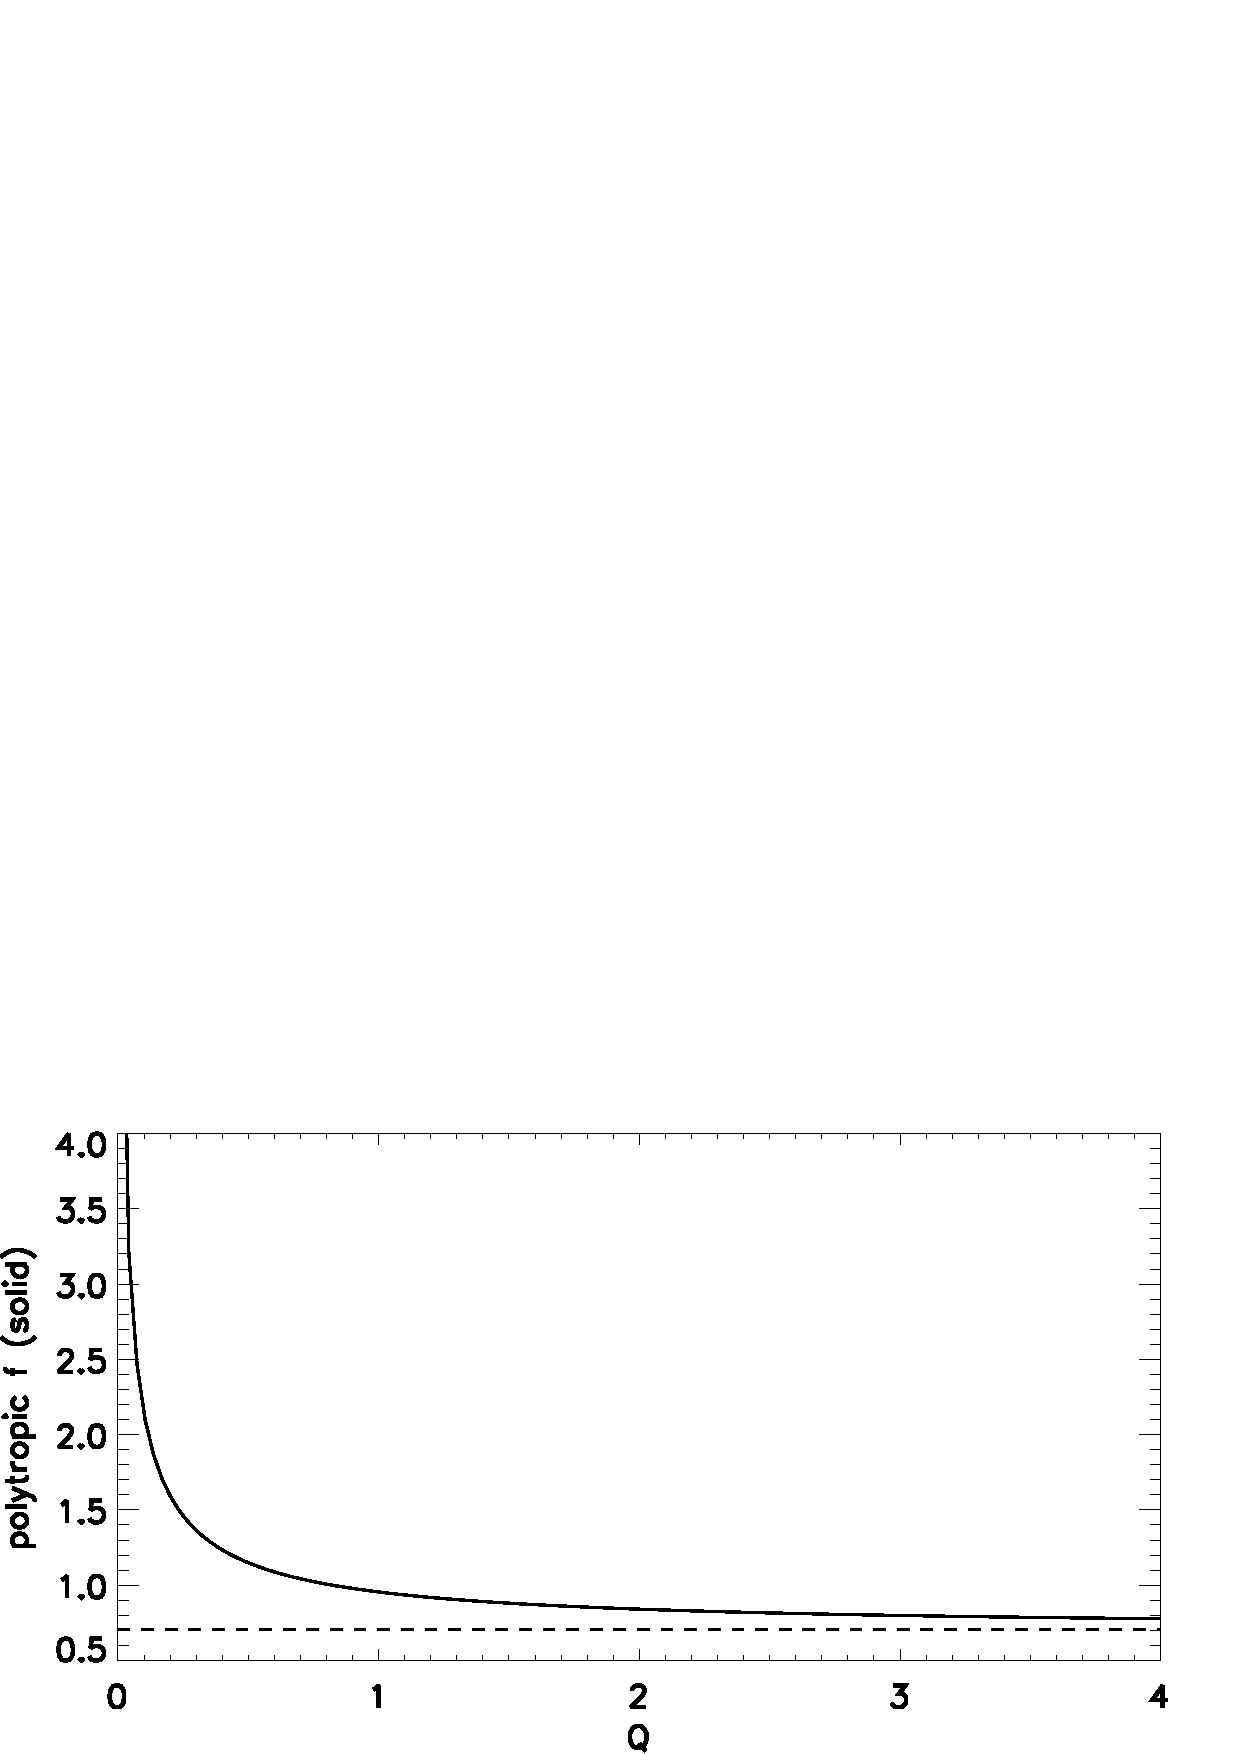
\includegraphics[width=\linewidth]{figures/plot_fq}
  \caption{The function $f(Q)$ describing vertical hydrodstatic 
    equilibrium in self-gravitating polytropic disks (solid line). The
    horizontal dashed line is the asymptotic value of $1/\sqrt{2}$ for
    large $Q$.  
    \label{plot_fq}}
\end{figure}


\section{Reduction to linear hydrodynamics}\label{reduction} 
Our task here is to remove the magnetic field and vertical velocity
perturbations from the non-dimensional linearized equations. 
Let us first define operators
\begin{align}
  D_0 = 1, \quad D_1 = \frac{\rho^\prime}{\rho} + \frac{d}{dz}, \quad
  D_2 = \frac{\rho^{\prime\prime}}{\rho} +
  \frac{2\rho^\prime}{\rho}\frac{d}{dz} + \frac{d^2}{d z^2},
\end{align}
and 
\begin{align}
  \overline{D}_0 = \eta D_0, \quad \overline{D}_1 = \eta^\prime D_0 + \eta
  D_1,\quad \overline{D}_2 = \eta^{\prime\prime} D_0 + 2\eta^\prime D_1 +
  \eta D_2. 
\end{align}
Denoting the $n^\mathrm{th}$ vertical derivative as $^{(n)}$, the
equations of motion give
\begin{align}
  &\dbx^{(n)} = \frac{\beta\rho}{f}D_{n-1}\left(\imgi\sigma\dvx - 2\dvy +
  \imgi f k_x\w\right) + \imgi k_x \dbz^{(n-1)},\label{bx_eq}\\
  &\dby^{(n)} = \frac{\beta\rho}{f}D_{n-1}\left(\imgi\sigma\dvy +
  \frac{\kappa^2}{2}\dvx\right),\label{by_eq}
\end{align}
for $n\geq1$. Differentiating the divergence-free condition for the magnetic
field gives
\begin{align}
  \imgi k_x \dbx^{\prime} + \dbz^{\prime\prime} = 0.   
\end{align}
We insert the expression for $\dbx^\prime$ from Eq. \ref{bx_eq} and the
expressoin for $\dbz^{\prime\prime}$ from the $z$ component of the
linearized induction equation (Eq. \ref{induct_vert}) to obtain
\begin{align}\label{bz_eq}
  -\sigma\dbz^{(n)} = f k_x \dvx^{(n)} + \frac{k_x\beta\rho}{f}\overline{D}_n\left(\imgi\sigma\dvx - 2\dvy +
  \imgi f k_x\w \right). 
\end{align}

\subsection{Eliminating $\dbx$}
Inserting the above expressions for $\dbx^{\prime\prime}$,
$\dbx^\prime$ (Eq. \ref{bx_eq}) and $\dbz^\prime$  (Eq. \ref{bz_eq})
into the right-hand-side of the $x$-induction equation (Eq. \ref{induct_x} ) gives   
\begin{align}
  \imgi\sigma \frac{f}{\beta\rho}\dbx =
  \frac{f^2}{\beta\rho}\dvx^\prime + \overline{D}_1\left(\imgi\sigma\dvx -
  2\dvy + \imgi f k_x\w\right). \label{bx_expression}
\end{align}
($\bar{\sigma}\neq0$ has been assumed to obtain this.) 
We multiply this expression by $\rho$, differentiate with respect to
$z$ and eliminate the resulting $\dbx^\prime$ using
Eq. \ref{bx_eq}, to obtain
\begin{align}
  0 = \frac{f^2}{\beta\rho}\dvx^{\prime\prime} -
  \frac{f^2}{\beta\rho}k_x^2\dvx + \left(\overline{D}_2 - k_x^2 \overline{D}_0
    - \imgi\sigma D_0\right)\left( \imgi\sigma\dvx -
  2\dvy + \imgi f k_x\w\right). \label{final_vx} 
\end{align}

\subsection{Eliminating $\dby$}
We follow a similar procedure as above to remove $\dby$. We first use
the divergence-free condition to eliminate $\dbx$ from the
right-hand-side of the $y$-induction equation (Eq. \ref{induct_y}),
\begin{align}
  &\imgi\bar{\sigma}\dby = f\dvy^\prime - \imgi
  S\frac{\dbz^\prime}{k_x} +
  \eta\dby^{\prime\prime}+\eta^\prime\dby^\prime.  
\end{align}
We can now insert expressions for the magnetic field derivatives using
Eq. \ref{by_eq} and \ref{bz_eq} to obtain an expression for $\dby$, 
\begin{align}
  \imgi\bar{\sigma}\dby = f \dvy^\prime + \frac{\imgi S}{\sigma}\left[
    f\dvx^\prime + \frac{\beta\rho}{f}\overline{D}_1\left(\imgi\sigma\dvx -
  2\dvy + \imgi f k_x\w \right)\right] +
  \frac{\beta\rho}{f}\overline{D}_1\left(\imgi\sigma\dvy +
  \frac{\kappa^2}{2}\dvx\right). \label{by_expression}
\end{align}
We differentiate this expression with respect to $z$, then eliminate 
$\dby$ and  $\dby^\prime$ from the left-hand-side of the resulting
expression using Eq. \ref{by_expression} and 
Eq. \ref{by_eq}, respectively. We obtain
\begin{align}
  0 =& \frac{f^2}{\beta\rho}\left(\dvy^{\prime\prime} -
  \frac{\bar{\sigma}^\prime}{\bar{\sigma}}\dvy^\prime\right) 
  + \sbar\sigma D_0\dvy  + \frac{\imgi 
    S}{\sigma}\frac{f^2}{\beta\rho}\left(\dvx^{\prime\prime} -
    \frac{\sbar^\prime}{\sbar}\dvx^\prime\right) -
    \frac{\imgi\sbar\kappa^2}{2}D_0\dvx \notag\\
    & + \left(\overline{D}_2 -
    \frac{\sbar^\prime}{\sbar}\overline{D}_1\right)\left[\imgi\left(\sigma
      - \frac{2S}{\sigma}\right)\dvy + \left(\frac{\kappa^2}{2} -
      S\right)\dvx - \frac{Sfk_x}{\sigma}\w\right]. \label{final_vy}
\end{align}

\subsection{Elminating $\dvz$}
The vertical velocity perturbation is
\begin{align}
  \dvz = \frac{\imgi f}{\sigma}\w^\prime. 
\end{align}
Inserting this into the linearized continuity equation
(Eq. \ref{lin_cont}) and using the Poisson equation, we obtain
\begin{align}
0=  W^{\prime\prime} + \left(\ln{\rho}\right)^\prime W^\prime +
  \frac{1}{c_s^2f^2}\left(\frac{\rho}{Q} + \sigma^2\right)W +
  \left(\ln{\rho}\right)^\prime\dphi^\prime + k_x^2\dphi + \frac{\sigma
  k_x}{f}\dvx.\label{final_w}
\end{align}
